\PassOptionsToPackage{unicode=true}{hyperref} % options for packages loaded elsewhere
\PassOptionsToPackage{hyphens}{url}
%
\documentclass[]{article}
\usepackage{lmodern}
\usepackage{amssymb,amsmath}
\usepackage{ifxetex,ifluatex}
\usepackage{fixltx2e} % provides \textsubscript
\ifnum 0\ifxetex 1\fi\ifluatex 1\fi=0 % if pdftex
  \usepackage[T1]{fontenc}
  \usepackage[utf8]{inputenc}
  \usepackage{textcomp} % provides euro and other symbols
\else % if luatex or xelatex
  \usepackage{unicode-math}
  \defaultfontfeatures{Ligatures=TeX,Scale=MatchLowercase}
\fi
% use upquote if available, for straight quotes in verbatim environments
\IfFileExists{upquote.sty}{\usepackage{upquote}}{}
% use microtype if available
\IfFileExists{microtype.sty}{%
\usepackage[]{microtype}
\UseMicrotypeSet[protrusion]{basicmath} % disable protrusion for tt fonts
}{}
\IfFileExists{parskip.sty}{%
\usepackage{parskip}
}{% else
\setlength{\parindent}{0pt}
\setlength{\parskip}{6pt plus 2pt minus 1pt}
}
\usepackage{hyperref}
\hypersetup{
            pdftitle={Branch length evaluation for Phylogenetic Diversity: a worked example},
            pdfauthor={Daniel R. Miranda-Esquivel},
            pdfborder={0 0 0},
            breaklinks=true}
\urlstyle{same}  % don't use monospace font for urls
\usepackage[margin=1in]{geometry}
\usepackage{color}
\usepackage{fancyvrb}
\newcommand{\VerbBar}{|}
\newcommand{\VERB}{\Verb[commandchars=\\\{\}]}
\DefineVerbatimEnvironment{Highlighting}{Verbatim}{commandchars=\\\{\}}
% Add ',fontsize=\small' for more characters per line
\usepackage{framed}
\definecolor{shadecolor}{RGB}{248,248,248}
\newenvironment{Shaded}{\begin{snugshade}}{\end{snugshade}}
\newcommand{\AlertTok}[1]{\textcolor[rgb]{0.94,0.16,0.16}{#1}}
\newcommand{\AnnotationTok}[1]{\textcolor[rgb]{0.56,0.35,0.01}{\textbf{\textit{#1}}}}
\newcommand{\AttributeTok}[1]{\textcolor[rgb]{0.77,0.63,0.00}{#1}}
\newcommand{\BaseNTok}[1]{\textcolor[rgb]{0.00,0.00,0.81}{#1}}
\newcommand{\BuiltInTok}[1]{#1}
\newcommand{\CharTok}[1]{\textcolor[rgb]{0.31,0.60,0.02}{#1}}
\newcommand{\CommentTok}[1]{\textcolor[rgb]{0.56,0.35,0.01}{\textit{#1}}}
\newcommand{\CommentVarTok}[1]{\textcolor[rgb]{0.56,0.35,0.01}{\textbf{\textit{#1}}}}
\newcommand{\ConstantTok}[1]{\textcolor[rgb]{0.00,0.00,0.00}{#1}}
\newcommand{\ControlFlowTok}[1]{\textcolor[rgb]{0.13,0.29,0.53}{\textbf{#1}}}
\newcommand{\DataTypeTok}[1]{\textcolor[rgb]{0.13,0.29,0.53}{#1}}
\newcommand{\DecValTok}[1]{\textcolor[rgb]{0.00,0.00,0.81}{#1}}
\newcommand{\DocumentationTok}[1]{\textcolor[rgb]{0.56,0.35,0.01}{\textbf{\textit{#1}}}}
\newcommand{\ErrorTok}[1]{\textcolor[rgb]{0.64,0.00,0.00}{\textbf{#1}}}
\newcommand{\ExtensionTok}[1]{#1}
\newcommand{\FloatTok}[1]{\textcolor[rgb]{0.00,0.00,0.81}{#1}}
\newcommand{\FunctionTok}[1]{\textcolor[rgb]{0.00,0.00,0.00}{#1}}
\newcommand{\ImportTok}[1]{#1}
\newcommand{\InformationTok}[1]{\textcolor[rgb]{0.56,0.35,0.01}{\textbf{\textit{#1}}}}
\newcommand{\KeywordTok}[1]{\textcolor[rgb]{0.13,0.29,0.53}{\textbf{#1}}}
\newcommand{\NormalTok}[1]{#1}
\newcommand{\OperatorTok}[1]{\textcolor[rgb]{0.81,0.36,0.00}{\textbf{#1}}}
\newcommand{\OtherTok}[1]{\textcolor[rgb]{0.56,0.35,0.01}{#1}}
\newcommand{\PreprocessorTok}[1]{\textcolor[rgb]{0.56,0.35,0.01}{\textit{#1}}}
\newcommand{\RegionMarkerTok}[1]{#1}
\newcommand{\SpecialCharTok}[1]{\textcolor[rgb]{0.00,0.00,0.00}{#1}}
\newcommand{\SpecialStringTok}[1]{\textcolor[rgb]{0.31,0.60,0.02}{#1}}
\newcommand{\StringTok}[1]{\textcolor[rgb]{0.31,0.60,0.02}{#1}}
\newcommand{\VariableTok}[1]{\textcolor[rgb]{0.00,0.00,0.00}{#1}}
\newcommand{\VerbatimStringTok}[1]{\textcolor[rgb]{0.31,0.60,0.02}{#1}}
\newcommand{\WarningTok}[1]{\textcolor[rgb]{0.56,0.35,0.01}{\textbf{\textit{#1}}}}
\usepackage{graphicx,grffile}
\makeatletter
\def\maxwidth{\ifdim\Gin@nat@width>\linewidth\linewidth\else\Gin@nat@width\fi}
\def\maxheight{\ifdim\Gin@nat@height>\textheight\textheight\else\Gin@nat@height\fi}
\makeatother
% Scale images if necessary, so that they will not overflow the page
% margins by default, and it is still possible to overwrite the defaults
% using explicit options in \includegraphics[width, height, ...]{}
\setkeys{Gin}{width=\maxwidth,height=\maxheight,keepaspectratio}
\setlength{\emergencystretch}{3em}  % prevent overfull lines
\providecommand{\tightlist}{%
  \setlength{\itemsep}{0pt}\setlength{\parskip}{0pt}}
\setcounter{secnumdepth}{0}
% Redefines (sub)paragraphs to behave more like sections
\ifx\paragraph\undefined\else
\let\oldparagraph\paragraph
\renewcommand{\paragraph}[1]{\oldparagraph{#1}\mbox{}}
\fi
\ifx\subparagraph\undefined\else
\let\oldsubparagraph\subparagraph
\renewcommand{\subparagraph}[1]{\oldsubparagraph{#1}\mbox{}}
\fi

% set default figure placement to htbp
\makeatletter
\def\fps@figure{htbp}
\makeatother


\title{Branch length evaluation for Phylogenetic Diversity: a worked example}
\author{Daniel R. Miranda-Esquivel}
\date{2020 - 10 - 11}

\begin{document}
\maketitle

\hypertarget{four-taxa-and-two-areas}{%
\section{Four taxa and two areas}\label{four-taxa-and-two-areas}}

\hypertarget{preparing-the-data-space}{%
\subsection{Preparing the data space}\label{preparing-the-data-space}}

First, we load the required libraries:

\begin{Shaded}
\begin{Highlighting}[]
\CommentTok{## cleaning}
\KeywordTok{rm}\NormalTok{(}\DataTypeTok{list =} \KeywordTok{ls}\NormalTok{())}

\CommentTok{## libraries}

\CommentTok{## installing and loading the package}

\CommentTok{##install.packages("../../blepd_0.mainRev.minorRev.tar.gz", repos = NULL, type="source")}

\KeywordTok{library}\NormalTok{(blepd)}
\end{Highlighting}
\end{Shaded}

\begin{verbatim}
## Loading required package: ape
\end{verbatim}

\begin{verbatim}
## Loading required package: picante
\end{verbatim}

\begin{verbatim}
## Loading required package: vegan
\end{verbatim}

\begin{verbatim}
## Loading required package: permute
\end{verbatim}

\begin{verbatim}
## 
## Attaching package: 'permute'
\end{verbatim}

\begin{verbatim}
## The following object is masked from 'package:devtools':
## 
##     check
\end{verbatim}

\begin{verbatim}
## Loading required package: lattice
\end{verbatim}

\begin{verbatim}
## This is vegan 2.5-6
\end{verbatim}

\begin{verbatim}
## Loading required package: nlme
\end{verbatim}

\begin{Shaded}
\begin{Highlighting}[]
\KeywordTok{packageVersion}\NormalTok{(}\StringTok{"blepd"}\NormalTok{)}
\end{Highlighting}
\end{Shaded}

\begin{verbatim}
## [1] '0.1.6.2020.10.11'
\end{verbatim}

\begin{Shaded}
\begin{Highlighting}[]
\CommentTok{## To plot trees you can use ggtree, ape or phytools. The example is based on}
\CommentTok{## ggtree as a matter of choice.}

\CommentTok{## More about ggtree}
\CommentTok{## https://guangchuangyu.github.io/ggtree-book/chapter-ggtree.html}

\CommentTok{## If you want to install ggtree go to}
\CommentTok{## https://bioconductor.org/packages/release/bioc/html/ggtree.html}

\KeywordTok{library}\NormalTok{(ggplot2)}

\KeywordTok{library}\NormalTok{(ggtree)}
\end{Highlighting}
\end{Shaded}

\begin{verbatim}
## Registered S3 method overwritten by 'treeio':
##   method     from
##   root.phylo ape
\end{verbatim}

\begin{verbatim}
## ggtree v2.2.4  For help: https://yulab-smu.github.io/treedata-book/
## 
## If you use ggtree in published research, please cite the most appropriate paper(s):
## 
## - Guangchuang Yu. Using ggtree to visualize data on tree-like structures. Current Protocols in Bioinformatics, 2020, 69:e96. doi:10.1002/cpbi.96
## - Guangchuang Yu, Tommy Tsan-Yuk Lam, Huachen Zhu, Yi Guan. Two methods for mapping and visualizing associated data on phylogeny using ggtree. Molecular Biology and Evolution 2018, 35(12):3041-3043. doi:10.1093/molbev/msy194
## - Guangchuang Yu, David Smith, Huachen Zhu, Yi Guan, Tommy Tsan-Yuk Lam. ggtree: an R package for visualization and annotation of phylogenetic trees with their covariates and other associated data. Methods in Ecology and Evolution 2017, 8(1):28-36. doi:10.1111/2041-210X.12628
\end{verbatim}

\begin{verbatim}
## 
## Attaching package: 'ggtree'
\end{verbatim}

\begin{verbatim}
## The following object is masked from 'package:nlme':
## 
##     collapse
\end{verbatim}

\begin{verbatim}
## The following object is masked from 'package:ape':
## 
##     rotate
\end{verbatim}

\begin{Shaded}
\begin{Highlighting}[]
\KeywordTok{library}\NormalTok{(gridExtra)}

\KeywordTok{library}\NormalTok{(RColorBrewer)}
\end{Highlighting}
\end{Shaded}

Now, we load the data included in the package: tree and distribution.

\begin{Shaded}
\begin{Highlighting}[]
\CommentTok{#data(package = "blepd")}

\CommentTok{## trees}

\KeywordTok{data}\NormalTok{(tree)}

\KeywordTok{str}\NormalTok{(tree)}
\end{Highlighting}
\end{Shaded}

\begin{verbatim}
## List of 5
##  $ edge       : int [1:6, 1:2] 5 6 6 5 7 7 6 1 2 7 ...
##  $ edge.length: num [1:6] 1 1 1 1 1 1
##  $ Nnode      : int 3
##  $ tip.label  : chr [1:4] "t1" "t2" "t3" "t4"
##  $ root.edge  : num 1
##  - attr(*, "class")= chr "phylo"
##  - attr(*, "order")= chr "cladewise"
\end{verbatim}

\begin{Shaded}
\begin{Highlighting}[]
\NormalTok{initialTree <-}\StringTok{ }\NormalTok{tree}


\CommentTok{## distributions}

\KeywordTok{data}\NormalTok{(distribution)}

\KeywordTok{str}\NormalTok{(distribution)}
\end{Highlighting}
\end{Shaded}

\begin{verbatim}
##  int [1:2, 1:4] 1 0 0 1 1 0 0 1
##  - attr(*, "dimnames")=List of 2
##   ..$ : chr [1:2] "A1" "A2"
##   ..$ : chr [1:4] "t1" "t2" "t3" "t4"
\end{verbatim}

\begin{Shaded}
\begin{Highlighting}[]
\NormalTok{dist4taxa <-}\StringTok{ }\NormalTok{distribution}

\CommentTok{## distribution to XY to be able to plot the data, otherwise skip the next step}

\NormalTok{distXY <-}\StringTok{ }\KeywordTok{matrix2XY}\NormalTok{(dist4taxa)}


\CommentTok{## plotting}

\CommentTok{## the tree}

\NormalTok{plotTree <-}\StringTok{  }\KeywordTok{ggtree}\NormalTok{(initialTree, }\DataTypeTok{ladderize=}\OtherTok{TRUE}\NormalTok{,}
                    \DataTypeTok{color=}\StringTok{"black"}\NormalTok{, }\DataTypeTok{size=}\DecValTok{1}\NormalTok{, }\DataTypeTok{linetype=}\StringTok{"dotted"}\NormalTok{) }\OperatorTok{+}
\StringTok{             }\KeywordTok{geom_tiplab}\NormalTok{(}\DataTypeTok{size=}\DecValTok{6}\NormalTok{, }\DataTypeTok{color=}\StringTok{"black"}\NormalTok{) }\OperatorTok{+}
\StringTok{             }\KeywordTok{theme_tree2}\NormalTok{() }\OperatorTok{+}
\StringTok{             }\KeywordTok{ggtitle}\NormalTok{(}\StringTok{"Four terminals, equal branch length"}\NormalTok{)}


\CommentTok{##print(plotTree)}



\CommentTok{## the distribution}

\NormalTok{plotDistrib <-}\StringTok{ }\KeywordTok{ggplot}\NormalTok{(}\DataTypeTok{data=}\NormalTok{distXY,}
                      \KeywordTok{aes}\NormalTok{(}\DataTypeTok{x=}\NormalTok{ Area, }\DataTypeTok{y=}\NormalTok{ Terminal),}
                      \DataTypeTok{size =}\DecValTok{11}\NormalTok{) }\OperatorTok{+}
\StringTok{               }\KeywordTok{geom_point}\NormalTok{() }\OperatorTok{+}
\StringTok{               }\KeywordTok{labs}\NormalTok{(}\DataTypeTok{title =} \StringTok{"Distributions"}\NormalTok{,}
                    \DataTypeTok{y =} \StringTok{""}\NormalTok{,}
                    \DataTypeTok{x =} \StringTok{"Area"}\NormalTok{)}

\CommentTok{##print(plotDistrib)}

\NormalTok{cowplot}\OperatorTok{::}\KeywordTok{plot_grid}\NormalTok{(plotTree, plotDistrib, }\DataTypeTok{ncol=}\DecValTok{2}\NormalTok{)}
\end{Highlighting}
\end{Shaded}

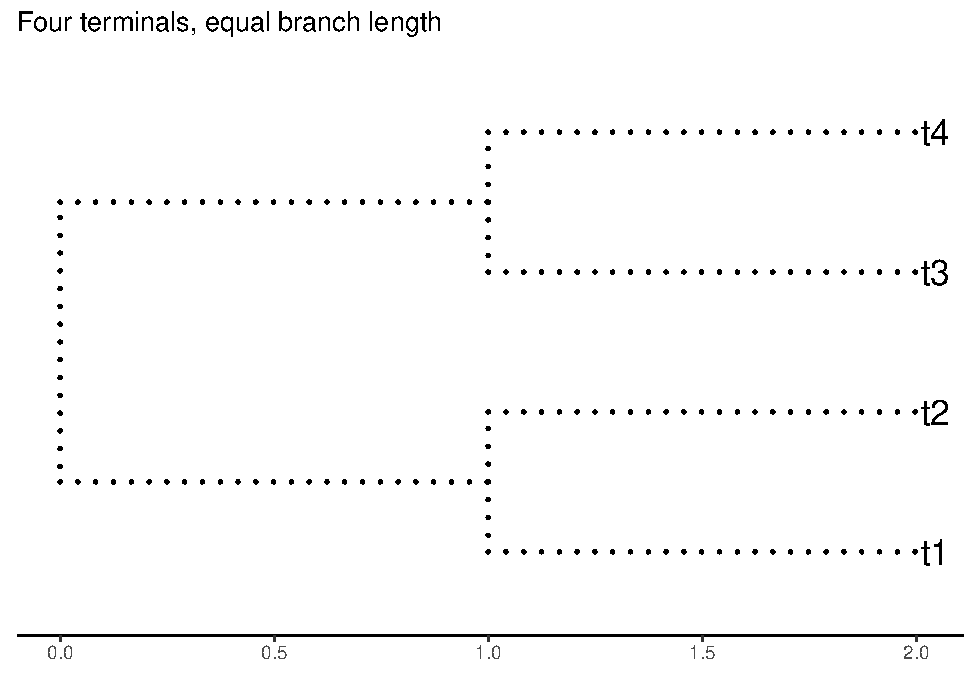
\includegraphics{workedExample_files/figure-latex/unnamed-chunk-2-1.pdf}

We check whether names in both objects: initialTree and dist4taxa, are
the same.

\begin{Shaded}
\begin{Highlighting}[]
\KeywordTok{all}\NormalTok{(}\KeywordTok{colnames}\NormalTok{(dist4taxa) }\OperatorTok{==}\StringTok{ }\NormalTok{initialTree}\OperatorTok{$}\NormalTok{tip.label)}
\end{Highlighting}
\end{Shaded}

\begin{verbatim}
## [1] TRUE
\end{verbatim}

We report the branch length, and calculate the PD values.

\begin{Shaded}
\begin{Highlighting}[]
\NormalTok{initialTree}\OperatorTok{$}\NormalTok{edge.length}
\end{Highlighting}
\end{Shaded}

\begin{verbatim}
## [1] 1 1 1 1 1 1
\end{verbatim}

\begin{Shaded}
\begin{Highlighting}[]
\NormalTok{initialPD <-}\StringTok{ }\KeywordTok{PDindex}\NormalTok{(}\DataTypeTok{tree=}\NormalTok{initialTree, }\DataTypeTok{distribution =}\NormalTok{ dist4taxa)}

\NormalTok{initialPD}
\end{Highlighting}
\end{Shaded}

\begin{verbatim}
## [1] 4 4
\end{verbatim}

As expected there is a tie between both areas.

\hypertarget{branch-swap}{%
\subsection{branch swap}\label{branch-swap}}

An initial approach, is to evaluate the effect in PD when internal and
terminal branch lengths are swapped. In this case it is not the
sensitivity to the branch length as a parameter, but the stability to
the actual branch lengths.

The function to perform the analysis is \emph{swapBL}, that has four
parameters: the tree, the distribution, the model to evaluate (valid
models are ``simpleswap'', ``allswap'' -default value- and ``uniform''),
the number of times to swap (default value = 100), and branch to swap
(``terminals'' (default) or ``internals'').

Uning the default parameters we get.

\begin{Shaded}
\begin{Highlighting}[]
\KeywordTok{swapBL}\NormalTok{(}\DataTypeTok{tree =}\NormalTok{ initialTree,}
       \DataTypeTok{distribution =}\NormalTok{ dist4taxa)}
\end{Highlighting}
\end{Shaded}

\begin{verbatim}
## model to test allswap reps 100
\end{verbatim}

\begin{verbatim}
## $initialPD
## [1] 4 4
## 
## $bestInitialArea
## [1] "A1A2"
## 
## $bestModifiedArea
##   AreaSelected Freq
## 1         A1A2  100
## 
## $tree
## 
## Phylogenetic tree with 4 tips and 3 internal nodes.
## 
## Tip labels:
##   t1, t2, t3, t4
## 
## Rooted; includes branch lengths.
## 
## $distribution
##    t1 t2 t3 t4
## A1  1  0  1  0
## A2  0  1  0  1
## 
## $model
## [1] "allswap"
## 
## $nTimes
## [1] 100
## 
## $root
## [1] TRUE
## 
## $index
## [1] "PD"
## 
## $branch
## [1] "terminals"
## 
## attr(,"class")
## [1] "blepd"
\end{verbatim}

As this is a tree where all branches are equal, there is no impact when
the branch lengths are swapped.

Or we could use the random uniform branch length model.

\begin{Shaded}
\begin{Highlighting}[]
\KeywordTok{swapBL}\NormalTok{(}\DataTypeTok{tree =}\NormalTok{ initialTree,}
       \DataTypeTok{distribution =}\NormalTok{ dist4taxa,}
       \DataTypeTok{model =} \StringTok{"uniform"}\NormalTok{)}
\end{Highlighting}
\end{Shaded}

\begin{verbatim}
## model to test uniform reps 100
\end{verbatim}

\begin{verbatim}
## $initialPD
## [1] 4 4
## 
## $bestInitialArea
## [1] "A1A2"
## 
## $bestModifiedArea
##   AreaSelected Freq
## 1         A1A2  100
## 
## $tree
## 
## Phylogenetic tree with 4 tips and 3 internal nodes.
## 
## Tip labels:
##   t1, t2, t3, t4
## 
## Rooted; includes branch lengths.
## 
## $distribution
##    t1 t2 t3 t4
## A1  1  0  1  0
## A2  0  1  0  1
## 
## $model
## [1] "uniform"
## 
## $nTimes
## [1] 100
## 
## $root
## [1] TRUE
## 
## $index
## [1] "PD"
## 
## $branch
## [1] "terminals"
## 
## attr(,"class")
## [1] "blepd"
\end{verbatim}

This is a tree where all branches are equal, therefore min and max are
equal. There is no impact when the branch lengths are swapped, and areas
A1A2 are selected.

\hypertarget{function-to-evaluate-a-single-terminal}{%
\subsection{Function to evaluate a single
terminal}\label{function-to-evaluate-a-single-terminal}}

To test the effect of changing the branch length in a single terminal
(``t1''), we will use the function \textbf{evalTerminal}. This function
uses four parameters: tree, distribution, tipToEval (label of the tip),
approach (two options: ``lower''/``upper'', to evaluate from 0 to the
actual length or from the actual length to the sum of all branch
lengths).

The function reports a S3 object, printable with \textbf{print.blepd}.

\begin{Shaded}
\begin{Highlighting}[]
\NormalTok{terminalT1 <-}\StringTok{ }\KeywordTok{evalTerminal}\NormalTok{(}\DataTypeTok{tree =}\NormalTok{ initialTree,}
             \DataTypeTok{distribution =}\NormalTok{ dist4taxa,}
             \DataTypeTok{tipToEval =} \StringTok{"t1"}\NormalTok{,}
             \DataTypeTok{approach =} \StringTok{"lower"}\NormalTok{ )}

\KeywordTok{print.blepd}\NormalTok{(terminalT1)}
\end{Highlighting}
\end{Shaded}

\begin{verbatim}
## 
## BestInitial:A1A2     Selected:   [1] "A2"
\end{verbatim}

\begin{Shaded}
\begin{Highlighting}[]
\NormalTok{terminalT1}\OperatorTok{$}\NormalTok{delta}
\end{Highlighting}
\end{Shaded}

\begin{verbatim}
## [1] 0.9999
\end{verbatim}

The lower limit reported when we change the branch length for terminal
t1 is 0.99 {[}stored as *object\textbf{\$delta}{]}, therefore, this
branch length will modify the area selected from A1A2 to A2, as the tie
between the path between terminals t1/t3 (area A1) vs t2/t4 (area A2)
will be solved in favour of t2/t4 when A1 is shorter.

In the same way, if we chage t1 to 1.01 the will break in favour of the
area A1.

\hypertarget{tree-evaluation-function}{%
\subsection{Tree evaluation function}\label{tree-evaluation-function}}

\hypertarget{branch-length}{%
\subsubsection{branch length}\label{branch-length}}

The function to test all terminals at the same time is \emph{evalTree},
with two parameters: the tree and the distribution. The function returns
a data.frame object with 14 fields: labelTerminal, lowerBranchLength,
InitialArea, lowerFinalArea, initialLength, upperBranchLength,
upperFinalArea, changeLower, changeUpper, deltaUpper, deltaLower,
deltaPD, areaDelta, and abDelta.

\begin{Shaded}
\begin{Highlighting}[]
\NormalTok{finalResults <-}\StringTok{   }\KeywordTok{evalTree}\NormalTok{(}\DataTypeTok{tree =}\NormalTok{ initialTree, }\DataTypeTok{distribution =}\NormalTok{ dist4taxa)}
\end{Highlighting}
\end{Shaded}

\begin{verbatim}
## Warning in `[<-.data.frame`(`*tmp*`, counter, c(2:5), value = structure(list(:
## replacement element 3 has 2 rows to replace 1 rows
\end{verbatim}

\begin{verbatim}
## Warning in `[<-.data.frame`(`*tmp*`, counter, c(2:5), value = structure(list(:
## replacement element 4 has 4 rows to replace 1 rows
\end{verbatim}

\begin{verbatim}
## Warning in `[<-.data.frame`(`*tmp*`, counter, c(2:5), value = structure(list(:
## replacement element 7 has 2 rows to replace 1 rows
\end{verbatim}

\begin{verbatim}
## Warning in `[<-.data.frame`(`*tmp*`, counter, c(2:5), value = structure(list(:
## replacement element 8 has 2 rows to replace 1 rows
\end{verbatim}

\begin{verbatim}
## Warning in `[<-.data.frame`(`*tmp*`, counter, c(2:5), value = structure(list(:
## provided 13 variables to replace 4 variables
\end{verbatim}

\begin{verbatim}
## Warning in `[<-.data.frame`(`*tmp*`, counter, c(6, 7), value = list(maxPD = 0, :
## replacement element 2 has 2 rows to replace 1 rows
\end{verbatim}

\begin{verbatim}
## Warning in `[<-.data.frame`(`*tmp*`, counter, c(2:5), value = structure(list(:
## replacement element 3 has 2 rows to replace 1 rows
\end{verbatim}

\begin{verbatim}
## Warning in `[<-.data.frame`(`*tmp*`, counter, c(2:5), value = structure(list(:
## replacement element 4 has 4 rows to replace 1 rows
\end{verbatim}

\begin{verbatim}
## Warning in `[<-.data.frame`(`*tmp*`, counter, c(2:5), value = structure(list(:
## replacement element 7 has 2 rows to replace 1 rows
\end{verbatim}

\begin{verbatim}
## Warning in `[<-.data.frame`(`*tmp*`, counter, c(2:5), value = structure(list(:
## replacement element 8 has 2 rows to replace 1 rows
\end{verbatim}

\begin{verbatim}
## Warning in `[<-.data.frame`(`*tmp*`, counter, c(2:5), value = structure(list(:
## provided 13 variables to replace 4 variables
\end{verbatim}

\begin{verbatim}
## Warning in `[<-.data.frame`(`*tmp*`, counter, c(6, 7), value = list(maxPD = 0, :
## replacement element 2 has 2 rows to replace 1 rows
\end{verbatim}

\begin{verbatim}
## Warning in `[<-.data.frame`(`*tmp*`, counter, c(2:5), value = structure(list(:
## replacement element 3 has 2 rows to replace 1 rows
\end{verbatim}

\begin{verbatim}
## Warning in `[<-.data.frame`(`*tmp*`, counter, c(2:5), value = structure(list(:
## replacement element 4 has 4 rows to replace 1 rows
\end{verbatim}

\begin{verbatim}
## Warning in `[<-.data.frame`(`*tmp*`, counter, c(2:5), value = structure(list(:
## replacement element 7 has 2 rows to replace 1 rows
\end{verbatim}

\begin{verbatim}
## Warning in `[<-.data.frame`(`*tmp*`, counter, c(2:5), value = structure(list(:
## replacement element 8 has 2 rows to replace 1 rows
\end{verbatim}

\begin{verbatim}
## Warning in `[<-.data.frame`(`*tmp*`, counter, c(2:5), value = structure(list(:
## provided 13 variables to replace 4 variables
\end{verbatim}

\begin{verbatim}
## Warning in `[<-.data.frame`(`*tmp*`, counter, c(6, 7), value = list(maxPD = 0, :
## replacement element 2 has 2 rows to replace 1 rows
\end{verbatim}

\begin{verbatim}
## Warning in `[<-.data.frame`(`*tmp*`, counter, c(2:5), value = structure(list(:
## replacement element 3 has 2 rows to replace 1 rows
\end{verbatim}

\begin{verbatim}
## Warning in `[<-.data.frame`(`*tmp*`, counter, c(2:5), value = structure(list(:
## replacement element 4 has 4 rows to replace 1 rows
\end{verbatim}

\begin{verbatim}
## Warning in `[<-.data.frame`(`*tmp*`, counter, c(2:5), value = structure(list(:
## replacement element 7 has 2 rows to replace 1 rows
\end{verbatim}

\begin{verbatim}
## Warning in `[<-.data.frame`(`*tmp*`, counter, c(2:5), value = structure(list(:
## replacement element 8 has 2 rows to replace 1 rows
\end{verbatim}

\begin{verbatim}
## Warning in `[<-.data.frame`(`*tmp*`, counter, c(2:5), value = structure(list(:
## provided 13 variables to replace 4 variables
\end{verbatim}

\begin{verbatim}
## Warning in `[<-.data.frame`(`*tmp*`, counter, c(6, 7), value = list(maxPD = 0, :
## replacement element 2 has 2 rows to replace 1 rows
\end{verbatim}

\begin{verbatim}
## Warning in evalTree(tree = initialTree, distribution = dist4taxa): NAs
## introduced by coercion

## Warning in evalTree(tree = initialTree, distribution = dist4taxa): NAs
## introduced by coercion

## Warning in evalTree(tree = initialTree, distribution = dist4taxa): NAs
## introduced by coercion
\end{verbatim}

\begin{Shaded}
\begin{Highlighting}[]
\CommentTok{## todo: errors to correct evalTree}

\NormalTok{finalResults}
\end{Highlighting}
\end{Shaded}

\begin{verbatim}
##   labelTerminal InitialArea initialLength lowerFinalArea lowerBranchLength
## 1            t1      0.9999            NA             A1                 0
## 2            t2      0.9999            NA             A1                 0
## 3            t3      0.9999            NA             A1                 0
## 4            t4      0.9999            NA             A1                 0
##   changeLower deltaLower upperFinalArea upperBranchLength changeUpper
## 1          A1         NA             A1                 0          A1
## 2          A1         NA             A1                 0          A1
## 3          A1         NA             A1                 0          A1
## 4          A1         NA             A1                 0          A1
##   deltaUpper deltaPD    areaDelta abDelta
## 1         NA       0 L:_A1_/U:_A1       0
## 2         NA       0 L:_A1_/U:_A1       0
## 3         NA       0 L:_A1_/U:_A1       0
## 4         NA       0 L:_A1_/U:_A1       0
\end{verbatim}

The extreme sensitivity of the PD results to the terminal branch length
is seen in the column absolute length difference (=abDelta), as any
length change -larger than 0-, will modify the area selected.

We plot the results to see the effect in each terminal, as a table.

\begin{Shaded}
\begin{Highlighting}[]
\NormalTok{plotResults <-}\StringTok{ }\KeywordTok{ggplot}\NormalTok{(}\DataTypeTok{data=}\NormalTok{finalResults, }\KeywordTok{aes}\NormalTok{(}\DataTypeTok{x=}\NormalTok{ labelTerminal, }\DataTypeTok{y=}\NormalTok{ initialLength,}
                      \DataTypeTok{shape=}\StringTok{"Actual"}\NormalTok{,}
                      \DataTypeTok{colour=}\NormalTok{InitialArea)) }\OperatorTok{+}
\StringTok{               }\KeywordTok{geom_point}\NormalTok{(}\DataTypeTok{size=} \DecValTok{7}\NormalTok{) }\OperatorTok{+}
\StringTok{               }\KeywordTok{geom_point}\NormalTok{(}\KeywordTok{aes}\NormalTok{(}\DataTypeTok{x=}\NormalTok{ labelTerminal, }\DataTypeTok{y=}\NormalTok{ lowerBranchLength,}
                              \DataTypeTok{colour=}\NormalTok{lowerFinalArea,}
                              \DataTypeTok{shape=}\StringTok{"Lower_limit"}\NormalTok{), }\DataTypeTok{size=}\DecValTok{7}\NormalTok{) }\OperatorTok{+}
\StringTok{               }\KeywordTok{labs}\NormalTok{(}\DataTypeTok{title =} \StringTok{"Branch length change, lower limits. Equal branches."}\NormalTok{,}
                    \DataTypeTok{colour =} \StringTok{"Area selected"}\NormalTok{,}
                    \DataTypeTok{shape =} \StringTok{"Terminal branch length value"}\NormalTok{,}
                    \DataTypeTok{y =} \StringTok{"Terminal branch length"}\NormalTok{,}
                    \DataTypeTok{x =} \StringTok{"Terminal"}\NormalTok{)}

\KeywordTok{print}\NormalTok{(plotResults)}
\end{Highlighting}
\end{Shaded}

\begin{verbatim}
## Warning: Removed 4 rows containing missing values (geom_point).
\end{verbatim}

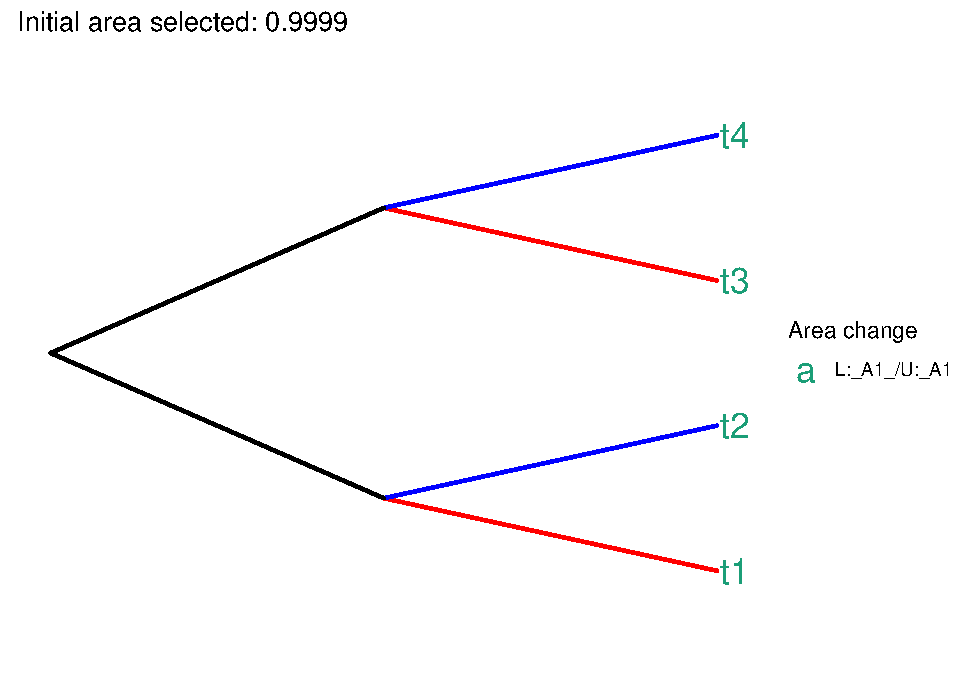
\includegraphics{workedExample_files/figure-latex/unnamed-chunk-9-1.pdf}

or plotted as a simple table.

\begin{Shaded}
\begin{Highlighting}[]
\NormalTok{countFreqChanges <-}\StringTok{ }\KeywordTok{table}\NormalTok{(finalResults}\OperatorTok{$}\NormalTok{areaDelta)}


\NormalTok{countFreqChanges <-}\StringTok{ }\KeywordTok{as.data.frame}\NormalTok{(countFreqChanges, }\DataTypeTok{ncol=}\DecValTok{1}\NormalTok{)}


\KeywordTok{colnames}\NormalTok{(countFreqChanges) <-}\StringTok{ }\KeywordTok{c}\NormalTok{(}\StringTok{"Area change"}\NormalTok{,}\StringTok{"Freq"}\NormalTok{)}


\KeywordTok{row.names}\NormalTok{(countFreqChanges) <-}\StringTok{ }\OtherTok{NULL}


\NormalTok{countFreqChanges}
\end{Highlighting}
\end{Shaded}

\begin{verbatim}
##    Area change Freq
## 1 L:_A1_/U:_A1    4
\end{verbatim}

or plotted into the tree:

\begin{Shaded}
\begin{Highlighting}[]
\NormalTok{theTitle <-}\StringTok{ }\KeywordTok{paste}\NormalTok{(}\StringTok{"Initial area selected:"}\NormalTok{,finalResults}\OperatorTok{$}\NormalTok{InitialArea[}\DecValTok{1}\NormalTok{])}

\NormalTok{p0 <-}\StringTok{    }\KeywordTok{ggtree}\NormalTok{(initialTree, }\DataTypeTok{layout=}\StringTok{"slanted"}\NormalTok{, }\DataTypeTok{ladderize=}\OtherTok{TRUE}\NormalTok{,}
                \DataTypeTok{color=}\KeywordTok{c}\NormalTok{(}\StringTok{"red"}\NormalTok{,}\StringTok{"blue"}\NormalTok{,}\StringTok{"red"}\NormalTok{,}\StringTok{"blue"}\NormalTok{,}\StringTok{"black"}\NormalTok{,}\StringTok{"black"}\NormalTok{,}\StringTok{"black"}\NormalTok{),}
                 \DataTypeTok{size=}\FloatTok{0.8}\NormalTok{ ) }\OperatorTok{+}
\StringTok{         }\KeywordTok{theme}\NormalTok{(}\DataTypeTok{legend.position=}\StringTok{"right"}\NormalTok{) }\OperatorTok{+}
\StringTok{         }\KeywordTok{labs}\NormalTok{(}\DataTypeTok{title =}\NormalTok{ theTitle)}


\NormalTok{p <-}\StringTok{ }\NormalTok{p0 }\OperatorTok\StringTok{ }\NormalTok{finalResults }\OperatorTok{+}\StringTok{ }\KeywordTok{geom_tiplab}\NormalTok{(}\KeywordTok{aes}\NormalTok{(}\DataTypeTok{color=}\NormalTok{areaDelta), }\DataTypeTok{size =}\DecValTok{6}\NormalTok{) }\OperatorTok{+}
\StringTok{          }\KeywordTok{scale_colour_brewer}\NormalTok{(}\StringTok{"Area change"}\NormalTok{, }\DataTypeTok{palette=}\StringTok{"Dark2"}\NormalTok{)}


\KeywordTok{print}\NormalTok{(p)}
\end{Highlighting}
\end{Shaded}

\includegraphics{workedExample_files/figure-latex/unnamed-chunk-11-1.pdf}

For terminals t1/t3, a change from 1 to 0.99 in branch length -the lower
limit (=L)- will change the initial area selected (A1A2) to A2; or a
change from 1 to 1.01 in branch length -the upper limit(=U)-, will
change the area to A1.

\end{document}
